\documentclass{beamer}
\usepackage{xmpmulti}
\usepackage{amsmath}
\usepackage{booktabs}
\usepackage{csquotes}% Recommended
\usepackage{natbib}
\usepackage{hyperref}
\usepackage{bbm}
\usepackage{comment}
\usepackage{bm}
\usepackage{makecell}
\usepackage{url}
\usepackage{colortbl}
\setbeamertemplate{footline}[frame number]
\setbeamertemplate{caption}[numbered]




\AtBeginSection[]{
    \begin{frame}
        \tableofcontents[currentsection]
    \end{frame}
}

\begin{comment}
    \AtBeginSubsection[]{
        \begin{frame}
            \tableofcontents[currentsection]
        \end{frame}
    }
\end{comment}


\title{The Cyclical Behavior of Equilibrium Unemployment and Vacancies\\
\citet{Shimer2005}}
\author{Presented by: XING Mingjie}
\date{\today}
\begin{document}

\begin{frame}
  \titlepage
\end{frame}

\begin{frame}{Bellman Equation}{Worker}
    \begin{itemize}
        \item Unempolyment value
            \begin{equation}\label{BellmanUnemploy}
                U_p = z + \delta \{f(\theta_p)\mathbb{E}_p W_{p^\prime} + (1-f(\theta_p))\mathbb{E}_p U_{p^\prime}\}
            \end{equation}
        \item Employment value
            \begin{equation}\label{BellmanEmploy}
                W_p = w_p + \delta \{(1-s)\mathbb{E}_p W_{p^\prime} + s\mathbb{E}_p U_{p^\prime}\}
            \end{equation}
    \end{itemize}
\end{frame}

\begin{frame}{Bellman Equation}{Firm}
    \begin{itemize}
        \item Hiring value
            \begin{equation}\label{BellmanHire}
                J_p = p - w_p + \delta (1-s)\mathbb{E}_p J_{p^\prime}
            \end{equation}
        \item Vacancy value
            \begin{equation}\label{BellmanVacancy}
                V_p = -c + \delta q(\theta_p)\mathbb{E}_p J_{p^\prime} \equiv 0
            \end{equation}
    \end{itemize}
\end{frame}

\begin{frame}{Productivity}
    The log of productivity follows AR(1) process
    \begin{equation}\label{productivityprocess}
    \log(p) = \rho \log(p) + \varepsilon 
    \end{equation}
    where \[\log(p) \sim N(\mu_\lambda, \sigma^2_\lambda),\ 
    \varepsilon \sim N(\mu_\varepsilon,\sigma^2_\varepsilon)\]
\end{frame}


\begin{frame}{Optimal Control}{Market tightness}
    \begin{itemize}
        \item Control in this problem consists of \(w_p, \theta_p, u_p\) and the state is \(p\)
        \item Market tightness \(\theta_p\) is given by solving the following equation of hire rate from free entry condition 
            \begin{equation}\label{HireRate}
            q(\theta_p) = \frac{c}{\delta \mathbb{E}_p J_{p^\prime}}\end{equation}
        \item And market tightness \begin{equation}
            \label{MarketTightness}
            \theta_p = (\frac{q(\theta_p)}{\mu})^{-\frac{1}{\eta}}
            \end{equation}
        \item Employ Rate is given by \begin{equation}\label{EmployRate}
            f(\theta_p) = \mu^\frac{1}{\eta} q^\frac{\eta-1}{\eta}
        \end{equation}
    \end{itemize}
\end{frame}

\begin{frame}{Optimal Control}{Continued}
    \begin{itemize}
        \item Optimal wage at each productivity level is given by the Nash Bargaining: 
        \begin{equation}\label{Nash}W_p - U_p = \beta (W_p - U_p + J_p)\end{equation}
        \item Note Bellman Equation of \(W_p\) given by \ref{BellmanEmploy}, \(U_p\) given by \ref{BellmanUnemploy}, \(J_p\) given by \ref{BellmanHire}
        \item Following the algebra given in slide \ref{OptWage}, optimal wage for each \(p\) is \begin{equation}\label{OptimalWage}
            w_p = \beta p + (1-\beta)z + \beta c \theta_p\end{equation}
        \item And unemployment rate \begin{equation}\label{UnemployRate}
            u_p = \frac{\delta}{\delta + f(\theta_p)}
        \end{equation}
    \end{itemize}
\end{frame}

\begin{frame}{Calibration}
    \begin{table}
        \begin{tabular}{
        >{\columncolor[HTML]{FFFFFF}}l 
        >{\columncolor[HTML]{FFFFFF}}l 
        >{\columncolor[HTML]{FFFFFF}}l }
        \hline
        Parameter         & Symbol                                                & Value \\ \hline
        Productivity std. & $\sigma_{logp}$                       & 0.05  \\
        Productivity mean & $\mu_{logp}$                          & 1     \\
        Stochastic std.   & $\sigma_{\varepsilon}$ & 0.03  \\
        Stochastic mean   & $\mu_{\varepsilon}$                    & 0     \\
        Separation rate   & $s$                                                     & 0.1   \\
        Discount rate     & $r$                                                     & 0.012 \\
        Value of leisure  & $z$                                                     & 0.4   \\
        Matching function & $\mu$                                                    & 1.355 \\
        Matching function & $\alpha$                                                 & 0.72  \\
        Bargaining Power  & $\beta$                                                  & 0.72  \\
        Cost of vacancy   & $c$                                                     & 0.213 \\ \hline
        \end{tabular}
        \caption{Parameter Calibration}
        \label{Calibration}
        \end{table}
\end{frame}

\begin{frame}[allowframebreaks]{Question a}{Discretization Algorithm}
    Inspired by Karen A. Kopecky 2006 Lecture Note
    \begin{enumerate}
        \item Choose a relateive error tolerance level \texttt{tol};
        \item Discretize the state space by constructing a grid for productivity \[
            p = \exp\{logp\}
            \text{\ where\ } logp = \{logp_1, logp_2, \ldots, logp_n\} \] given by the Tauchen-Hussey (1991) method.
            The n is chosen at 100;
        \item Start with an initial guess of the value function \(V^{(0)}(p)\) is a vector of length \(n\), i.e., \(V^{(0)}(p) = \{V^{(0)}_i\}_{i=1}^n\), where \(V^{(0)}_i = V^{(0)}(p_i)\).
            \(V\) here represents \(U, W, J\). The initial guess is ones.
        \framebreak
        \label{update}
        \item Update the value function using eqautions \ref{BellmanUnemploy} to \ref{OptimalWage}, specifically
            \begin{enumerate}
                \item Fix the current productivity level at one of the grid points, \(p_i\) from \(i=1\)
                \item For each possible choice of productivity next period, calculate optimal control in the following order:
                \begin{gather*}
                    q(\theta_{p_i}) = \frac{c}{\delta \sum_{j=1}^{n}p_{i,j}J^{(0)}(p_j)}\\
                    f(\theta_{p_i}) = \mu^\frac{1}{\eta} q^\frac{\eta-1}{\eta}\\
                    \theta_{p_i} = (\frac{q(\theta_{p_i})}{\mu})^{-\frac{1}{\eta}}\\
                    w_{p_i} = \beta p_i + (1-\beta)z + \beta c \theta_{p_i}
                \end{gather*}
                \item and update the value function system with 
                \framebreak
                \begin{gather*}
                    U^{(1)}_{p_i} = z + \delta\{f(\theta_{p_i})\sum_{j=1}^{n}p_{i,j}W^{(0)}(p_j) + (1-f(\theta_{p_i}))\sum_{j=1}^{n}p_{i,j}U^{(0)}(p_j)\}\\
                    W^{(1)}_{p_i} = w_{p_i} + \delta\{(1-s)\sum_{j=1}^{n}p_{i,j}W^{(0)}(p_j) + s\sum_{j=1}^{n}p_{i,j}U^{(0)}(p_j)\}\\
                    J^{(1)}_{p_i} = p_i - w_{p_i} + \delta (1-s)\sum_{j=1}^{n}p_{i,j}J^{(0)}(p_j)
                \end{gather*}
                \item Choose a new grid point for productivity, go through 4.1 to 4.3. Once we have done the update for all productivity grid, we have new system of value function \({V^{(1)}_p}\)
                \item Compute distance between the two systems of value functions following the sup norm \[
                    d = \max\limits_{i\in\{1,\ldots,n\}}|V^{(0)}_i-V^{(1)}_i|\]
                \framebreak
                \item If distance is within the error tolerance level, \(d \leq tol * ||V^{(1)}_1||\), the functions have converged and go to step 5, or else go back to step 4.
            \end{enumerate}
            \item Calculate the optimal control for each productivity level:
            \begin{gather*}
                q(\theta^*_{p_i}) = \frac{c}{\delta \sum_{j=1}^{n}p_{i,j}J^* (p_j)}\\
                f(\theta^*_{p_i}) = \mu^\frac{1}{\eta} q^\frac{\eta-1}{\eta}\\
                \theta^*_{p_i} = (\frac{q(\theta^*_{p_i})}{\mu})^{-\frac{1}{\eta}}\\
                w^*_{p_i} = \beta p_i + (1-\beta)z + \beta c \theta^*_{p_i}\\
                u^*_p = \frac{\delta}{\delta + f(\theta^*_p)}
            \end{gather*}
            where \(J^*\) is the converged value function.
    \end{enumerate}
\end{frame}


\begin{frame}{Tauchen-Hussey 1991}
    Use \texttt{discretizeAR1\_Tauchen} function from the Matlab Toolbox of \cite{Kirkby2023} .
\end{frame}

    
% \begin{frame}{Matlab Code}{Discretization Method}
    
% \end{frame}

\begin{frame}{Question a}{Parametric Approximation}
    \begin{enumerate}\addtocounter{enumi}{-1}
        \item Choose Hermite interpolation polynomials to approximate $\hat{V}(p;\textbf{coefs})$ in the form of \(
            f(x) = a (x-x_1)^3 + b(x-x_1)^2 + c(x-x_1)+d 
            \) with Matlab code \texttt{pchip}. Report initial paramters with \texttt{pp.coefs} for each value function, save as \texttt{old}
        \item Maximize control and calculate value function at each productivity level as done in Discretization method
        \item Fit for new value function system and report parameters and save as \texttt{new}
        \item If \(||\hat{V}(p;\textbf{coef\_sold})-\hat{V}(p;\textbf{coefs\_new})||<tol\), stop; else go to step 1.
    \end{enumerate}
\end{frame}

% \begin{frame}{Matlab Code}{Discretization Method}
    
% \end{frame}

% \begin{frame}{Optimal Controls from two methods}
%     \begin{figure}[ht]
%         \begin{minipage}[b]{0.45\linewidth}
%             \centering
%             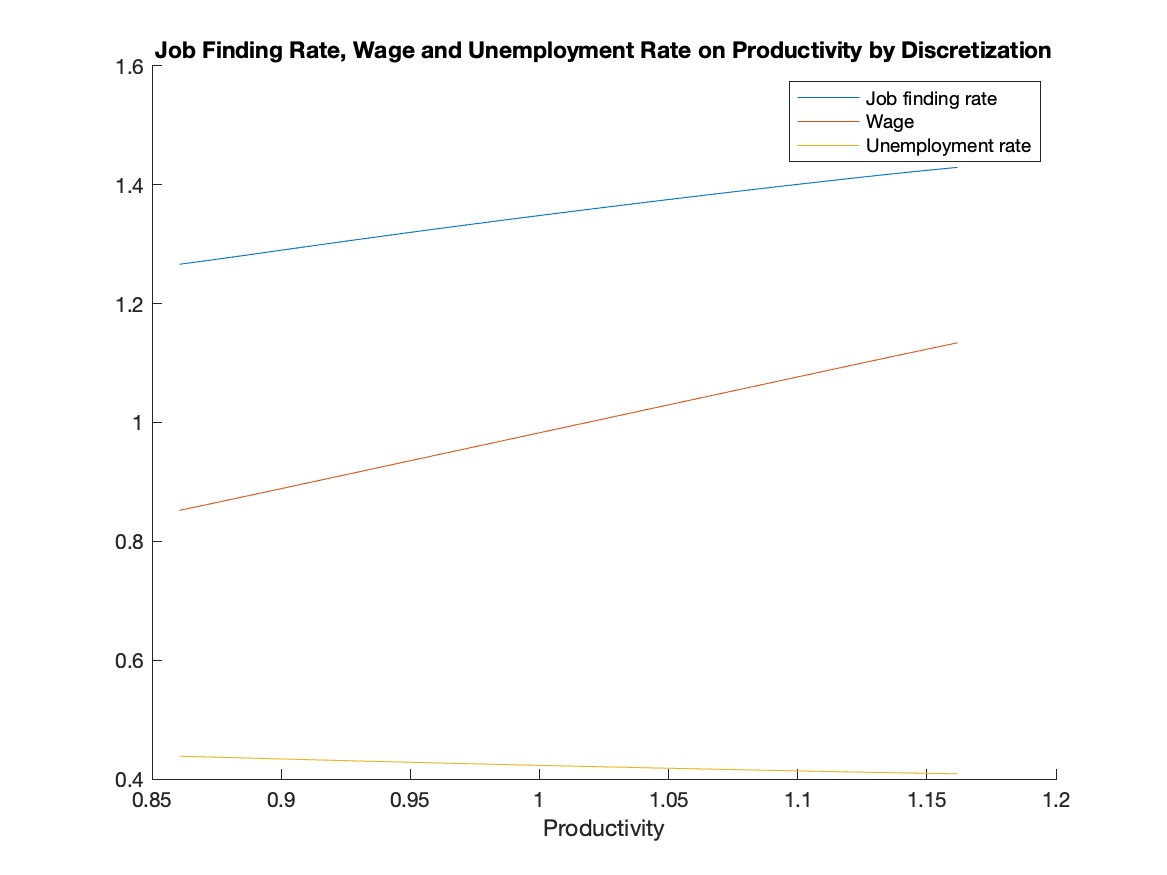
\includegraphics[width=\textwidth]{"/Users/mingjiexing/Desktop/HKU/Courses/6096_Computational_Method/Final/Shimer_2005/Discretization.jpg"}
%             \caption{Label for a}
%             \label{fig:a}
%         \end{minipage}
%         \hspace{0.5cm}
%         \begin{minipage}[b]{0.45\linewidth}
%             \centering
%             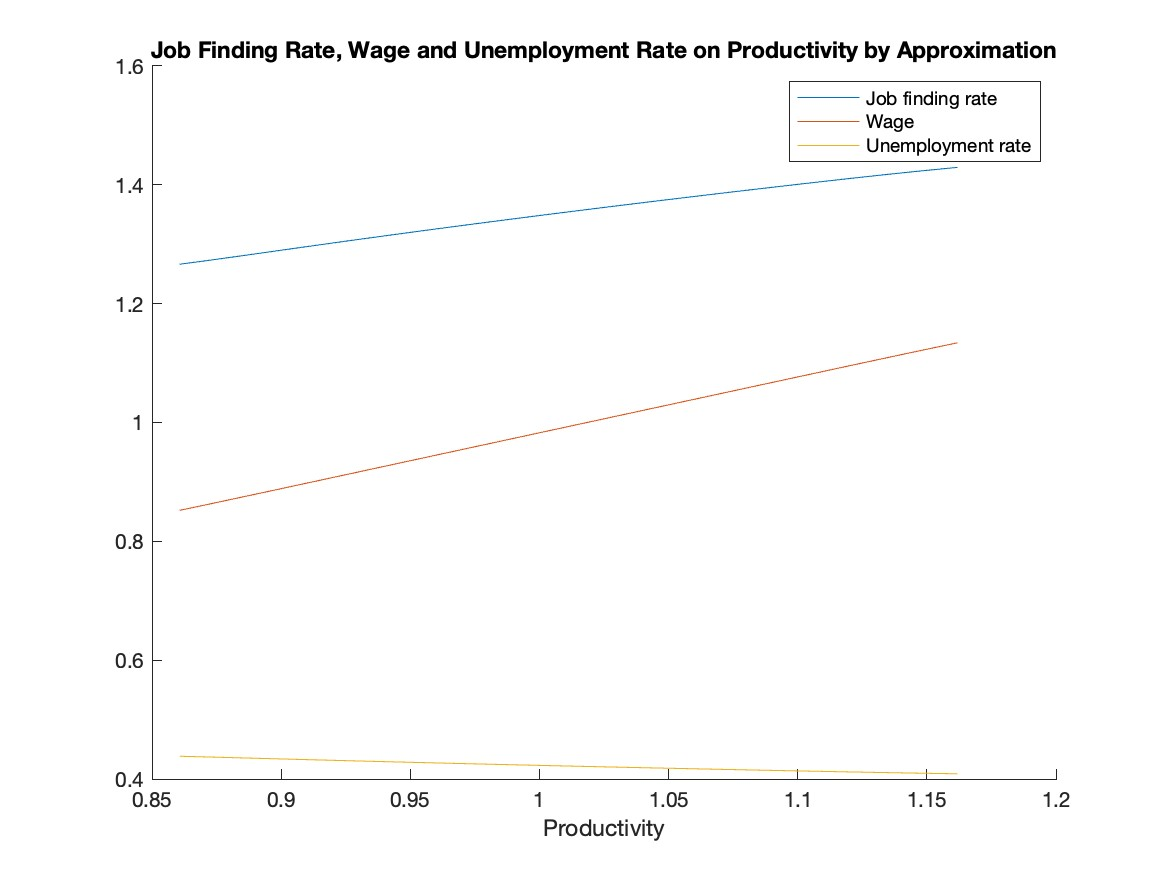
\includegraphics[width=\textwidth]{"/Users/mingjiexing/Desktop/HKU/Courses/6096_Computational_Method/Final/Shimer_2005/Approximation.jpg"}
%             \caption{Label for b}
%             \label{fig:b}
%         \end{minipage}
%     \end{figure}
% \end{frame}

\begin{frame}{Two Results}{Question b}
    To use the polynomial interpolation function from class directly
    \begin{table}[]
        \begin{tabular}{
        >{\columncolor[HTML]{FFFFFF}}l 
        >{\columncolor[HTML]{FFFFFF}}l 
        >{\columncolor[HTML]{FFFFFF}}l 
        >{\columncolor[HTML]{FFFFFF}}l }
        \hline
        log(p) & w & u & f \\ \hline
        0.400  &   &   &   \\
        0.700  &   &   &   \\
        1.000  &   &   &   \\
        1.300  &   &   &   \\
        1.600  &   &   &   \\ \hline
        \end{tabular}
        \caption{Wage, Unemployment rate and Job Finding Rate}
        \label{Qb}
        \end{table}
\end{frame}

\begin{frame}{Two Results}{Question c}
    \begin{table}[]
        \begin{tabular}{
        >{\columncolor[HTML]{FFFFFF}}l 
        >{\columncolor[HTML]{FFFFFF}}l 
        >{\columncolor[HTML]{FFFFFF}}l 
        >{\columncolor[HTML]{FFFFFF}}l }
        \hline
                                  & u     & f     & p     \\ \hline
        Data Std.                 & 0.190 & 0.118 & 0.020 \\
        Approximation Model Std.  &       &       &       \\
        Discretization Model Std. &       &       &       \\ \hline
        \end{tabular}
        \caption{Model fit on Unemployment, Job finding rate and productivity}
        \label{Qc}
        \end{table}
\end{frame}

\begin{frame}{Appendix A}{Optimal wage}\label{OptWage}
    \begin{gather*}
        W_p - U_p = \beta (W_p - U_p + J_p)\\
        \Leftrightarrow
        w_p - z + \delta (1-s-f(\theta_p))(\mathbb{E}_p W_{p^\prime}-\mathbb{E}_p U_{p^\prime}) =\\
        \beta (p-z+\delta (1-s-f(\theta_p))(\mathbb{E}_p W_{p^\prime}-\mathbb{E}_p U_{p^\prime}) +\delta(1-s)\mathbb{E}_p J_{p^\prime})\\
        \Leftrightarrow
        w_p = \beta p + (1-\beta)z + (\beta-1)\delta(1-s-f(\theta_p))(\mathbb{E}_p W_{p^\prime}-\mathbb{E}_p U_{p^\prime})\\
         + \frac{\beta c(1-s)}{q(\theta_p)}\\
        \Leftrightarrow
        w_p = \beta p + (1-\beta)z - \frac{\beta c\delta(1-s-f(\theta_p))}{q(\theta_p)} + \frac{\beta c(1-s)}{q(\theta_p)}\\
        \Leftrightarrow
        w_p = \beta p + (1-\beta)z + \beta c \theta_p
    \end{gather*}
    where we use the fact that \(\mathbb{E}_p W_{p^\prime}-\mathbb{E}_p U_{p^\prime} = \frac{\beta}{1-\beta}\mathbb{E}_p J_{p^\prime}\) and \(f(\theta_p)/q(\theta_p)=\theta_p\)
\end{frame}

\setbeamertemplate{footline}{}
\begin{frame}[allowframebreaks,noframenumbering]{Reference}
    \footnotesize
    \bibliographystyle{agsm}
\bibliography{Shimer2005}
\end{frame}
\end{document}